\documentclass[hyperref={colorlinks=true,citecolor=green,linkcolor=red}]{beamer}


\usepackage{algorithm}
\usepackage{algpseudocode}
\usepackage{graphicx}
\usepackage{amsmath}
\usepackage{amsthm} % theorem-like environments
\usepackage{subfig}
\usepackage[numbers,square]{natbib}
\usepackage[inactive,blur=0.6,fixcolor,preview]{fancytooltips}


\title{Minimal working example to test \texttt{fancy-preview}}
\date{}


\begin{document}
	
	
	
\begin{frame}
	\titlepage
\end{frame}


\begin{frame}
   \frametitle{Test slide}
   This slide is for the testing the various environments. Hover the mouse from the right to get the pop-up reference (needs to be opened in Adobe Reader).
   \begin{itemize}
      \item Testing citation: Article \cite{Bourdin2008}
      \item Testing equation: Equation \eqref{eq:EulerIdentity}
      \item Testing figure: Figure \ref{fig:testFig}
      \item Testing enumeration: Enumeration \ref{enum:testEnum}
      \item Testing algorithm: Algorithm \ref{alg:testAlg}
      \item Testing theorem: Theorem \ref{th:testTheorem}
   \end{itemize}
\end{frame}


\begin{frame}
   \frametitle{Equation}
   \begin{equation}
      e^{i\pi} + 1 = 0
      \label{eq:EulerIdentity}
   \end{equation}
\end{frame}


\begin{frame}
   \frametitle{Figure}
   \begin{figure}
      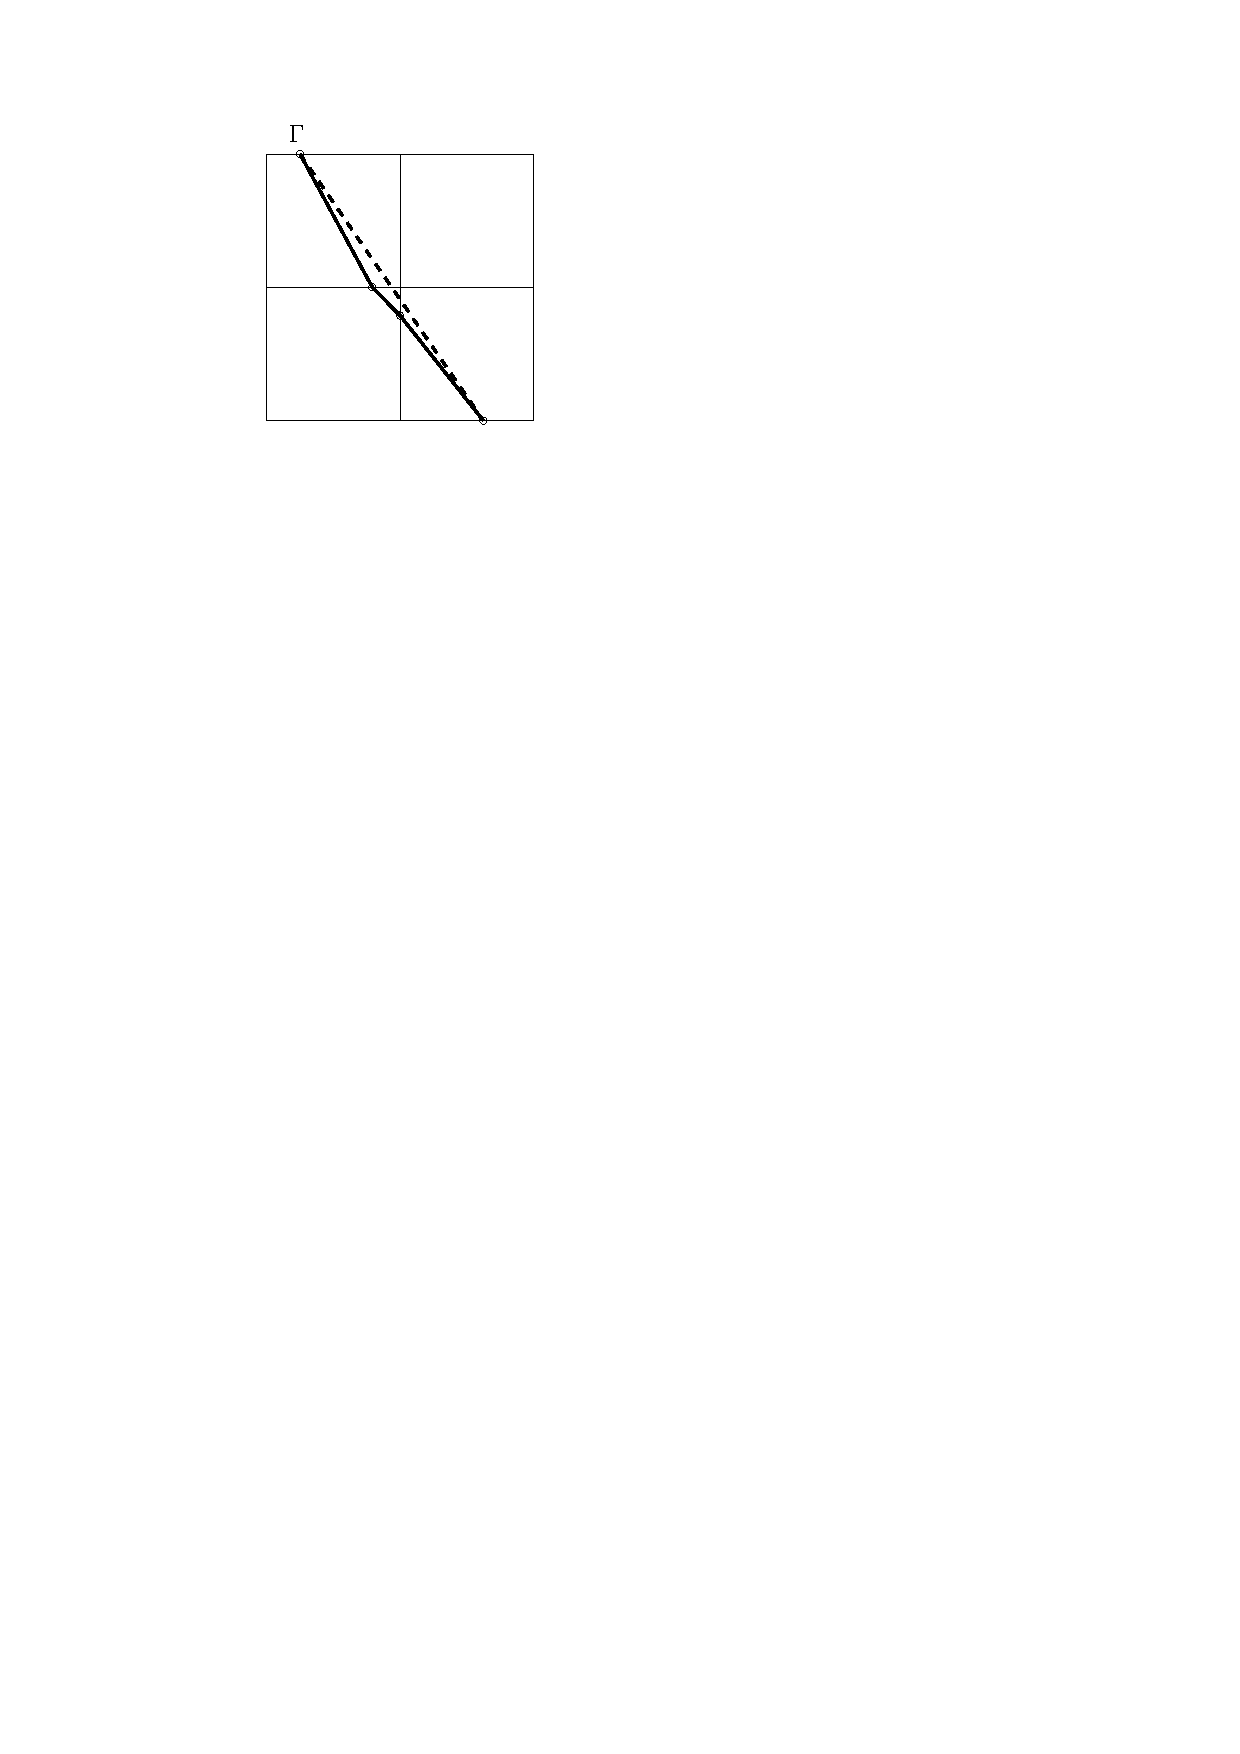
\includegraphics[scale=1]{testPicture.pdf}
      \caption{}
      \label{fig:testFig}
   \end{figure}
\end{frame}


\begin{frame}
   \frametitle{Enumeration}
   \begin{enumerate}
      \item First item
      \item Second item
      \label{enum:testEnum}
   \end{enumerate}
\end{frame}


\begin{frame}
   \frametitle{Algorithm}
   \begin{algorithm}[H]
      \caption{Factorial}
      \label{alg:testAlg}
      \begin{algorithmic}[1]
         \State $N = 10$ \Comment{Initialise loop count}
         \State \texttt{fac} $\gets 1$ \Comment{Set starting value, i.e. $0!$}
         \For {$i$ from 1 to $N$}
            \State \texttt{fac} $\gets$ \texttt{fac}*$i$
         \EndFor
      \end{algorithmic}
   \end{algorithm}
\end{frame}


\begin{frame}
   \frametitle{Theorem}
   \begin{theorem}
      No three positive integers $a$, $b$, and $c$ satisfy the equation $a^n + b^n = c^n$ for any integer value of $n$ greater than 2.
      \label{th:testTheorem}
   \end{theorem}
\end{frame}


\begin{frame}
   \frametitle{Reference}
   \bibliographystyle{abbrvnat}
   \bibliography{testReferences}
\end{frame}


\end{document}